%% Direttive TeXworks:
% !TeX root = ./presentazione.tex
% !TEX encoding = UTF-8 Unicode
% !TEX program = arara
% !TEX TS-program = arara
% !TeX spellcheck = it-IT

%! arara: clean: { files: [ arara.log, presentazione.aux, presentazione.log, presentazione.nav, presentazione.out, presentazione.snm, presentazione.toc, presentazione.xmpdata, pdfa.xmpi, presentazione.pdf ] }
% arara: clean: { files: [ arara.log, presentazione.log, presentazione.xmpdata, pdfa.xmpi, presentazione.pdf ] }
% arara: pdflatex: { shell: yes, synctex: yes, action: batchmode, options: "-halt-on-error -file-line-error-style" }
% arara: biber
% arara: pdflatex: { shell: yes, synctex: yes, action: batchmode, options: "-halt-on-error -file-line-error-style" }
% arara: pdflatex: { shell: yes, synctex: yes, action: nonstopmode, options: "-halt-on-error -file-line-error-style" }

%%%%%%%%%%%%%%%%%%%%%%%%%%%%%%%%%%%%%%%%%%%%%%%%%%%%%%%%
%% Genera un file report.xmpdata con i dati per PDF/A %%
\begin{filecontents*}{\jobname.xmpdata}
\Title{RxJS: Reactive Extensions For JavaScript}
\Author{Niccolò Maltoni}
\Copyright{Copyright \copyright 2018, Niccolò Maltoni}
\CopyrightURL{http://creativecommons.org/licenses/by-nc-sa/3.0/it/}
\Keywords{RxJS\sep ReactiveX\sep JavaScript\sep JS}
\end{filecontents*}
%%%%%%%%%%%%%%%%%%%%%%%%%%%%%%%%%%%%%%%%%%%%%%%%%%%%%%%%

\documentclass[%
    % handout             % configura la presentazione per la stampa
]{beamer}

%%%%%%%%%%%%%%%%%%%%%%%%%%%%%%%%%%%%%%%%%%%%%%%%%%%%%%%%%%%%
%% Imposto la codifica del sorgente e del testo in uscita %%
\usepackage[T1]{fontenc}        % serve per impostare la codifica di output del font
\usepackage{textcomp}           % serve per fornire supporto ai Text Companion fonts
 \usepackage[utf8]{inputenc}     % serve per impostare la codifica di input del font
\usepackage[
    english,            % utilizza l'inglese come lingua secondaria
    italian             % utilizza l'italiano come lingua primaria
]{babel}                        % serve per scrivere Indice, Capitolo, etc in Italiano
\usepackage{lmodern}            % carica una variante Latin Modern prodotto dal GUST
%%%%%%%%%%%%%%%%%%%%%%%%%%%%%%%%%%%%%%%%%%%%%%%%%%%%%%%%%%%%

\usepackage{graphicx}           % serve per includere immagini e grafici

\usepackage{tikz}
\usepackage{listings}
\usepackage{minted}
\usemintedstyle{native}
\definecolor{monokaibg}{RGB}{46,46,46}
\setminted[js]{fontsize=\scriptsize,linenos=true,bgcolor=monokaibg}

\usepackage[%
    strict,             % rende tutti gli warning degli errori
    autostyle,          % imposta lo stile in base al linguaggio specificato in babel
    english=american,   % imposta lo stile per l'inglese
    italian=guillemets  % imposta lo stile per l'italiano
]{csquotes}                     % serve a impostare lo stile delle virgolette

\usepackage[%
    maxcitenames=2,     % massimo numero di nomi nelle citazioni
    mincitenames=2,     % minimo numero di nomi nelle citazioni
    maxbibnames=99,     % massimo numero di nomi nella blibliografia
    minbibnames=99,     % minimo numero di nomi nella blibliografia
    style=numeric,
    giveninits=true,
    backend=biber       % specifica il backend per la bibliografia
]{biblatex}                     % si interfaccia con bibtex e biber per la bibliografia
\addbibresource{biblio.bib}

\graphicspath{{img/}}

\usepackage[%
    depth=3,            % equivale a bookmarksdepth di hyperref
    open=false,         % equivale a bookmarksopen di hyperref
    numbered=true       % equivale a bookmarksnumbered di hyperref
]{bookmark}                     % Gestisce i segnalibri meglio di hyperref
\hypersetup{%
    pdfpagemode={UseNone},
    hidelinks,          % nasconde i collegamenti (non vengono quadrettati)
    hypertexnames=false,
    linktoc=all,        % inserisce i link nell'indice
    plainpages=false,
    breaklinks,
    pdfstartview={Fit},
    unicode=true,       % only Latin characters in Acrobat's bookmarks
    pdftoolbar=false,   % show Acrobat's toolbar?
    pdfmenubar=false,   % show Acrobat's menu?
    plainpages=false
}
\usepackage{nameref}
\usepackage[pdf15,a-1b]{pdfx}

%%%%%%%%%%%%%%%%%%%%%%%%%%%
%% Impostazione del tema %%
\usetheme{Boadilla}             % serve per scegliere il layout generale dei frame
\definecolor{darkrxpurple}{RGB}{87,43,139}
\definecolor{rxpurple}{RGB}{216,26,96}
\colorlet{primarygrey}{gray!30!white}
\colorlet{secondarygrey}{gray!15!white}
\colorlet{terziarygrey}{gray!10!white}
\colorlet{greyrxpurple}{rxpurple!75!secondarygrey}
\definecolor{lighrxpurple}{RGB}{236,12,144}
\colorlet{greylightrxpurple}{lighrxpurple!25!terziarygrey}
\usecolortheme{beaver}          % Per il colore va comunque bene questo
% \usecolortheme[named=rxpurple]{structure}
\setbeamerfont{block title}{size=\normalsize}
\setbeamerfont{block body}{size=\small}
\setbeamertemplate{navigation symbols}{}  % nasconde i controlli di presentazione
\setbeamercolor{palette primary}{fg=darkrxpurple, bg=greylightrxpurple}
\setbeamercolor{palette secondary}{fg=white, bg=lighrxpurple}
\setbeamercolor{palette tertiary}{fg=white, bg=darkrxpurple}
% \setbeamercolor{title}{fg=white}
% \setbeamercolor{subtitle}{fg=white}
\setbeamercolor{title}{fg=white, bg=darkrxpurple}
\setbeamercolor{subtitle}{fg=white, bg=darkrxpurple}
\setbeamercolor{frametitle}{fg=rxpurple}
\setbeamercolor{framesubtitle}{fg=rxpurple}
\setbeamercolor{block title}{fg=darkrxpurple}

\renewcommand{\thefootnote}{\arabic{footnote}}
%%%%%%%%%%%%%%%%%%%%%%%%%%%

%%%%%%%%%%%%%%%%%%%%%%%%%%%%%%%%%%%%%%%%%%%%%%%%%%%%%%%%%%%%%%%%%%%%
%% Definisco un nuovo comando per enfatizzare il testo in inglese %%
\newcommand{\engEmph}[1] {\emph{\foreignlanguage{english}#1}}
%%%%%%%%%%%%%%%%%%%%%%%%%%%%%%%%%%%%%%%%%%%%%%%%%%%%%%%%%%%%%%%%%%%%

%%%%%%%%%%%%%%%%%%%%%%%%%%%%%%%%%%%%%%%%%%%%%%%%%%%%%%%%%%
%% Permette di inserire l'outline prima di ogni sezione %%
\AtBeginSection[]{%
    \begin{frame}<beamer>
        \frametitle{Outline}
        \tableofcontents[currentsection,subsubsectionstyle=hide]
    \end{frame}
}
%%%%%%%%%%%%%%%%%%%%%%%%%%%%%%%%%%%%%%%%%%%%%%%%%%%%%%%%%%

%%%%%%%%%%%%%%%%%%%%%%%%%%%%%%%%%%%%%%%%%%%%%%%%%%%%%%%%%%%%%%%
%% Permette di inserire automaticamente titolo e sottotitolo %%
% \addtobeamertemplate{frametitle}{
%    \let\insertframetitle\insertsectionhead}{}
% \addtobeamertemplate{frametitle}{
%    \let\insertframesubtitle\insertsubsectionhead}{}

% \makeatletter
%   \CheckCommand*\beamer@checkframetitle{\@ifnextchar\bgroup\beamer@inlineframetitle{}}
%   \renewcommand*\beamer@checkframetitle{\global\let\beamer@frametitle\relax\@ifnextchar\bgroup\beamer@inlineframetitle{}}
% \makeatother
%%%%%%%%%%%%%%%%%%%%%%%%%%%%%%%%%%%%%%%%%%%%%%%%%%%%%%%%%%%%%%%

\title[RxJS]{ReactiveX RxJS}
\subtitle{Reactive Extensions For JavaScript}
\author[Niccolò~Maltoni]{\large{Niccolò~Maltoni}\\{\small\texttt{niccolo.maltoni@studio.unibo.it}}}
\date[30 maggio 2018]{}
\institute[0000840825]{
\includegraphics[scale=.4]{Rx_Logo}}

\begin{document}
    \begin{frame}[c]
        \titlepage
    \end{frame}

    \section{Introduzione}\label{sec:intro}

        \subsection{Programmazione reattiva}\label{subsec:react}

        \begin{frame}{\insertsectionhead}
            \begin{block}{\insertsubsectionhead}
                \smallskip
                \begin{quote}
                    \foreignlanguage{english}
                    `` It is convenient to distinguish roughly between three kinds of computer programs.
                    Transformational programs compute results from a given set of inputs;
                    typical examples are compilers or numerical computation programs.
                    Interactive programs interact at their own speed with users or with other programs;
                    from a user point of view, a time-sharing system is interactive.
                    \textbf{Reactive programs also maintain a continuous interaction with their environment, but at a speed which is determined by the environment, not the program itself}.
                    Interactive programs work at their own pace and mostly deal with communication, while reactive programs only work in response to external demands and mostly deal with accurate interrupt handling. ''
                \end{quote}
                \rightline{Gérard~Berry,~1989~\cite{berry:inria-00075494}}
            \end{block}
        \end{frame}

        \subsection{Reactive Manifesto}\label{subsec:manifest}

        \begin{frame}{\insertsectionhead}
            \begin{block}{\insertsubsectionhead~\cite{citeulike:13845446}}
                \begin{itemize}
                    \item
                        Prima versione presentata nel 2013
                    \item
                        Principi base:
                        \begin{itemize}
                            \item \textbf{responsività}
                            \item \textbf{resilienza}
                            \item scalabilità
                            \item \engEmph{event-driven}
                        \end{itemize}
                    \item
                        La versione attuale (2.0) è stata presentata l'anno successivo\footnotemark
                        \begin{itemize}
                            \item da scalabilità a \textbf{elasticità}
                            \item da \engEmph{event-driven} a \textbf{\engEmph{message-driven}}
                        \end{itemize}
                \end{itemize}
            \end{block}
            \footnotetext{\url{https://www.lightbend.com/blog/reactive-manifesto-20}}
        \end{frame}

        \begin{frame}[c]{\insertsectionhead}{\insertsubsectionhead}
            \begin{figure}[htbp]
                \centering
                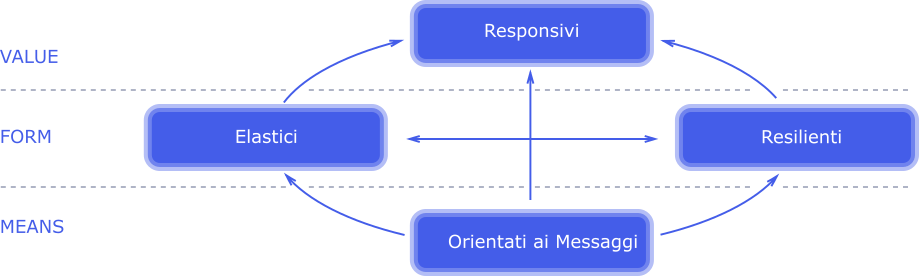
\includegraphics[width=\linewidth]{reactive-traits-it}
                \caption{Rappresentazione dei principi base del \engEmph{Reactive Manifesto}}
                \label{fig:manifest}
            \end{figure}
        \end{frame}

        \begin{frame}[c]{\insertsectionhead}{\insertsubsectionhead}
            \begin{columns}
                \begin{column}{.47\textwidth}
                    \centering
                    \subsubsection{Responsività}\label{subsub:responsive}
                    \begin{block}{\insertsubsubsectionhead}
                        \begin{itemize}
                            \item
                                \textbf{tempestività} della risposta
                                \begin{itemize}
                                {
                                    \footnotesize
                                    \item rapida identificazione dei problemi
                                    \item minimizzazione del tempo di risposta
                                }
                                \end{itemize}
                            \item
                                garanzia di \textbf{qualità del servizio} nel tempo
                            \item
                                \textbf{predicibilità} del comportamento
                                \begin{itemize}
                                {
                                    \footnotesize
                                    \item semplificazione della gestione degli errori
                                    \item fiducia degli utenti finali nel sistema
                                }
                                \end{itemize}
                        \end{itemize}
                    \end{block}
                \end{column}
                \begin{column}{.47\textwidth}
                    \centering
                    \subsubsection{Resilienza}\label{subsub:resiliency}
                    \begin{block}{\insertsubsubsectionhead}
                        \begin{itemize}
                            \item
                                il sistema resta \textbf{responsivo anche in caso di guasti}
                            \item
                                garantita tramite:
                                \begin{itemize}
                                {
                                    \footnotesize
                                    \item replica
                                    \item contenimento
                                    \item isolamento
                                    \item delega
                                }
                            \end{itemize}
                        \end{itemize}
                    \end{block}
                \end{column}
            \end{columns}
        \end{frame}

        \begin{frame}[c]{\insertsectionhead}{\insertsubsectionhead}
            \begin{columns}
                \begin{column}{.47\textwidth}
                    \centering
                    \subsubsection{Elasticità}\label{subsub:elasticity}
                    \begin{block}{\insertsubsubsectionhead}
                        \begin{itemize}
                            \item
                                il sistema rimane \textbf{responsivo sotto carichi di lavoro variabili} nel tempo
                            \item
                                \textbf{adattabilità} attraverso incremento o decremento delle risorse allocate al processamento degli input
                                \begin{itemize}
                                {
                                    \footnotesize
                                    \item no sezioni contese né colli di bottiglia
                                    \item distribuibilità
                                    \item replica dei componenti
                                    \item ripartizione degli input
                                }
                                \end{itemize}
                            \item possibile implementazione predittiva
                        \end{itemize}
                    \end{block}
                \end{column}
                \begin{column}{.47\textwidth}
                    \centering
                    \subsubsection{\engEmph{Message-Driven}}\label{subsub:meddagedriven}
                    \begin{block}{\insertsubsubsectionhead}
                        \begin{itemize}
                            \item
                                \textbf{scambio di messaggi asincrono}
                                \begin{itemize}
                                {
                                    \footnotesize
                                    \item stile di comunicazione non bloccante
                                }
                                \end{itemize}
                            \item
                                basso accoppiamento tra i componenti
                            \item
                                isolamento e trasparenza sul dislocamento
                            \item
                                esprimere i guasti del componente sotto forma di messaggi
                        \end{itemize}
                    \end{block}
                \end{column}
            \end{columns}
        \end{frame}

        \subsection{Reactive Extensions}\label{subsec:rx}

        \begin{frame}{\insertsectionhead}
            \begin{block}{\insertsubsectionhead}
                \begin{itemize}
                    \item
                        Reactive Extensions (o \textbf{ReactiveX}) sono un set di librerie per la maggior parte dei linguaggi e dei framework moderni che permette l'implementazione di programmi in grado di operare su sequenze di dati e input in modo \textit{reattivo} e \textit{asincrono}, indipendentemente dalla natura della sorgente
                    \item
                        ispirate alle \engEmph{Microsoft's Reactive Extensions} per ambiente .NET
                    \item
                        combinazione di:
                        \begin{itemize}
                        {
                            \footnotesize
                            \item pattern Observer
                            \item pattern Iterator
                            \item programmazione funzionale
                        }
                        \end{itemize}
                \end{itemize}
            \end{block}
            \begin{figure}[htbp]
                \centering
                
\includegraphics[scale=.35]{Rx_Logo_Text}
                \label{fig:rx}
            \end{figure}
        \end{frame}

    \section{RxJS: Reactive Extensions Library for JavaScript}\label{sec:rxjs}

        \subsection{Reactive Extensions per JavaScript (e TypeScript)}\label{subsec:rxjs}

        \begin{frame}[fragile]{\insertsectionhead}
            \begin{block}{\insertsubsectionhead\footnotemark}
                \begin{itemize}
                    \item
                        RxJS è una libreria per la programmazione reattiva pensata per JavaScript
                    \item
                        semplifica l'implementazione di \engEmph{callback} e chiamate asincrone attraverso il tipo \texttt{Observable} e i suoi costrutti satelliti, come:
                        \begin{itemize}
                            \item \texttt{Observer}
                            \item \texttt{Schedulers}
                            \item \texttt{Subjects}
                            \item operatori come \texttt{map}, \texttt{filter}, \texttt{reduce}, \texttt{every}, ecc ...
                        \end{itemize}
                \end{itemize}
            \end{block}
            \footnotetext{\url{http://reactivex.io/rxjs}}
        \end{frame}

        % \begin{frame}{\insertsectionhead}
        %     \subsubsection{Caratteristiche}\label{subsub:characteristics}
        %     \begin{block}{\insertsubsubsectionhead}
        %         \begin{itemize}
        %             \item
        %                 \engEmph{Purity} (purezza): è in grado di generare valori utilizzando funzioni pure
        %                 \begin{itemize}
        %                     \item codice meno propenso ad errori
        %                 \end{itemize}
        %             \item
        %                 \engEmph{Flow} (flusso): gli \texttt{Observable} permettono un controllo su un flusso di eventi e/o valori
        %             \item
        %                 \engEmph{Values} (valori): gli osservabili permettono di manipolare valori all'interno del flusso.
        %         \end{itemize}
        %     \end{block}
        % \end{frame}

        \begin{frame}[fragile]{\insertsectionhead}
        \subsubsection{Installazione}\label{subsec:install}
        \begin{block}{\insertsubsubsectionhead}
            \begin{itemize}
                \item
                    Via \textbf{\url{npm}}:
                    \inputminted[fontsize=\scriptsize]{text}{src/npm_install.sh}
                \item
                    Via \textbf{\footnotesize CDN}:
                    \inputminted[fontsize=\scriptsize]{text}{src/cdn_install.html}
            \end{itemize}
        \end{block}
        \end{frame}

        \subsection{Costrutti fondamentali}\label{subsec:costrutti}

            \subsubsection{Observable}\label{subsub:observable}

            \begin{frame}{\insertsubsectionhead}
                \begin{block}{\texttt{\insertsubsubsectionhead}}
                    \begin{itemize}
                        \item costituisce il costrutto base della libreria
                        \item è uno \engEmph{stream}, costruito in modo asincrono col procedere del tempo
                        \item è in grado di generare valori utilizzando funzioni pure
                        \item offre operatori per il controllo di flusso
                    \end{itemize}
                \end{block}
            \end{frame}

            \begin{frame}{\insertsubsectionhead}{\insertsubsubsectionhead}
                \begin{block}{Hot VS Cold}
                    \begin{itemize}
                        \item
                            Uno \engEmph{stream} si definisce \textbf{\engEmph{cold}} se l'\texttt{Observable} genera il produttore dei valori nel flusso; per esempio:

                            \inputminted{js}{src/cold_observable.js}

                        \item
                            Uno \engEmph{stream} si definisce \textbf{\engEmph{hot}} se l'\texttt{Observable} racchiude il produttore dei valori nel flusso; per esempio:

                            \inputminted{js}{src/hot_observable.js}
                    \end{itemize}
                \end{block}
            \end{frame}

            \subsubsection{.pipe()}\label{subsub:pipe}

            \begin{frame}{\insertsubsectionhead}{\nameref{subsub:observable}}
                \begin{block}{\texttt{\insertsubsubsectionhead}}<1->
                    \begin{itemize}
                        \item
                            A partire da RxJS 5.5, sono stati introdotti i \engEmph{pipable operators}
                        \item
                            da RxJS 6, essi sono gli operatori standard, trovabili in \texttt{rxjs/operators}
                        \item
                            l'operatore \texttt{.pipe()} prende un infinito numero di argomenti, che sono funzioni applicabili allo stream; ad esempio:

                            \inputminted{js}{src/pipe.js}
                            % \begin{figure}
                            %
                            %     \caption{Lo stream emette numeri incrementali ogni 350ms e completa dopo il 25° valore; essi sono mappati con una funzione gaussiana e convertiti in una serie di caratteri ``•''}
                            % \end{figure}

                    \end{itemize}
                \end{block}
                \only<2 | handout 0> {
                    \begin{tikzpicture}[remember picture,overlay]
                        \node[at=(current page.center)] {
                            
\includegraphics[width=.8\paperwidth, height=.8\paperheight]{pipe_meme}
                        };
                    \end{tikzpicture}
                }
            \end{frame}

            \subsubsection{.map()}\label{subsub:map}

            \begin{frame}{\insertsubsectionhead}{\nameref{subsub:observable}: Pipable operators}
                \begin{block}{\texttt{\insertsubsubsectionhead}}
                    \begin{itemize}
                        \item
                            simile alla funzione \texttt{.map()} degli array
                        \item
                            applica una \textbf{funzione proiezione} ad ogni valore emesso dall'\texttt{Observable} sorgente ed emette i valori risultanti come \texttt{Observable}
                        \item
                            utile per il parsing di JSON
                    \end{itemize}
                \end{block}

            \end{frame}

            \begin{frame}[fragile]{\insertsubsectionhead}{\nameref{subsub:observable}: Pipable operators: \texttt{\insertsubsubsectionhead}}
                \inputminted{js}{src/map.js}
                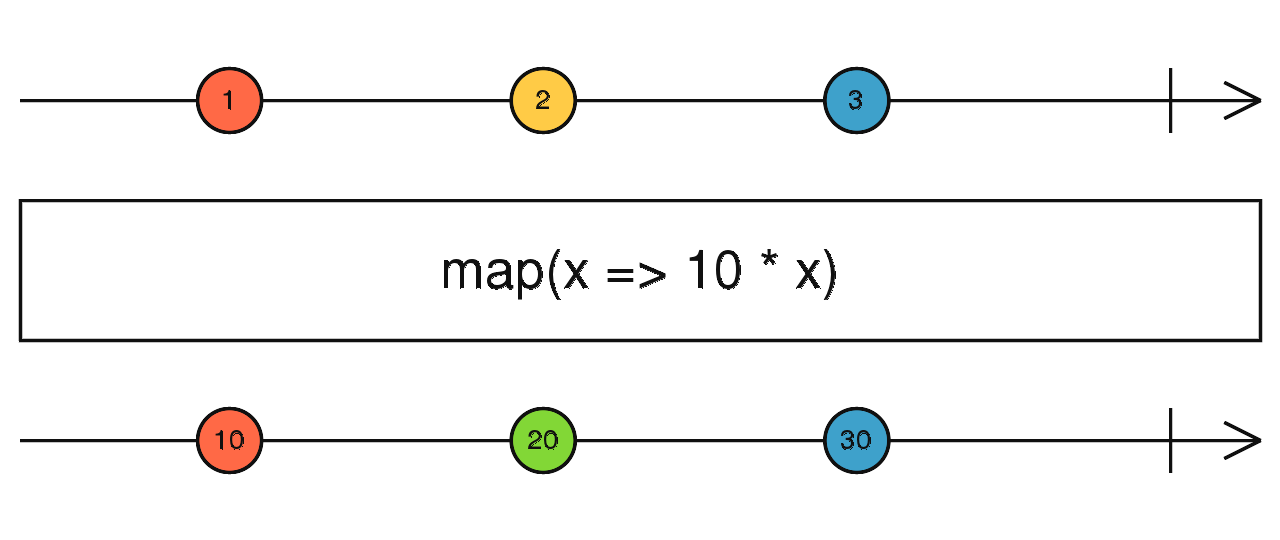
\includegraphics[width=\linewidth]{map}
            \end{frame}

            \subsubsection{.reduce() \& .scan()}\label{subsub:reduce}

            \begin{frame}{\insertsubsectionhead}{\nameref{subsub:observable}}
                \begin{block}{\texttt{.reduce()}}
                    \begin{itemize}
                        \item
                            simile alla funzione \texttt{.reduce()} degli array
                        \item
                            applica una \textbf{funzione accumulatore} sull'\texttt{Observable} sorgente e ritorna il risultato una volta che la sorgente termina
                    \end{itemize}
                \end{block}

                \begin{block}{\texttt{.scan()}}
                    \begin{itemize}
                        \item
                            applica una \textbf{funzione accumulatore} sull'\texttt{Observable} sorgente e ritorna ogni risultato intermedio
                        \item
                            simile alla \texttt{.reduce()}, ma emette un valore ad ogni valore emesso dalla sorgente anziché attenderne il completamento
                    \end{itemize}
                \end{block}

            \end{frame}

            \begin{frame}[fragile]{\insertsubsectionhead}{\nameref{subsub:observable}: Pipable operators: \texttt{\insertsubsubsectionhead}}
                \inputminted{js}{src/reduce.js}
                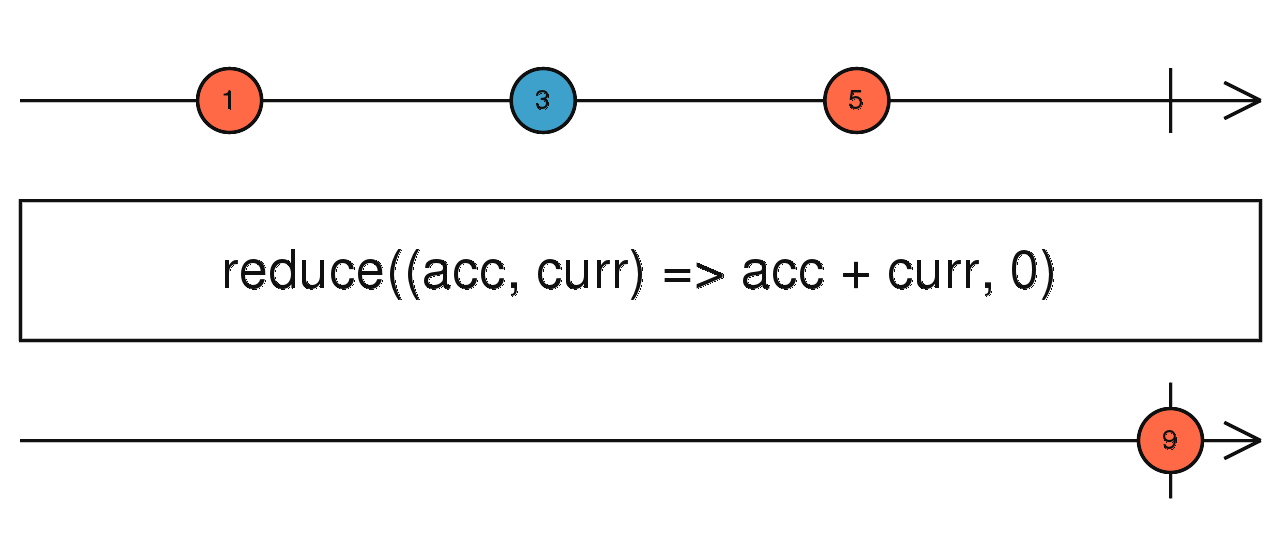
\includegraphics[width=\linewidth]{reduce}
            \end{frame}

            \begin{frame}[fragile]{\insertsubsectionhead}{\nameref{subsub:observable}: Pipable operators: \texttt{\insertsubsubsectionhead}}
                \inputminted{js}{src/scan.js}
                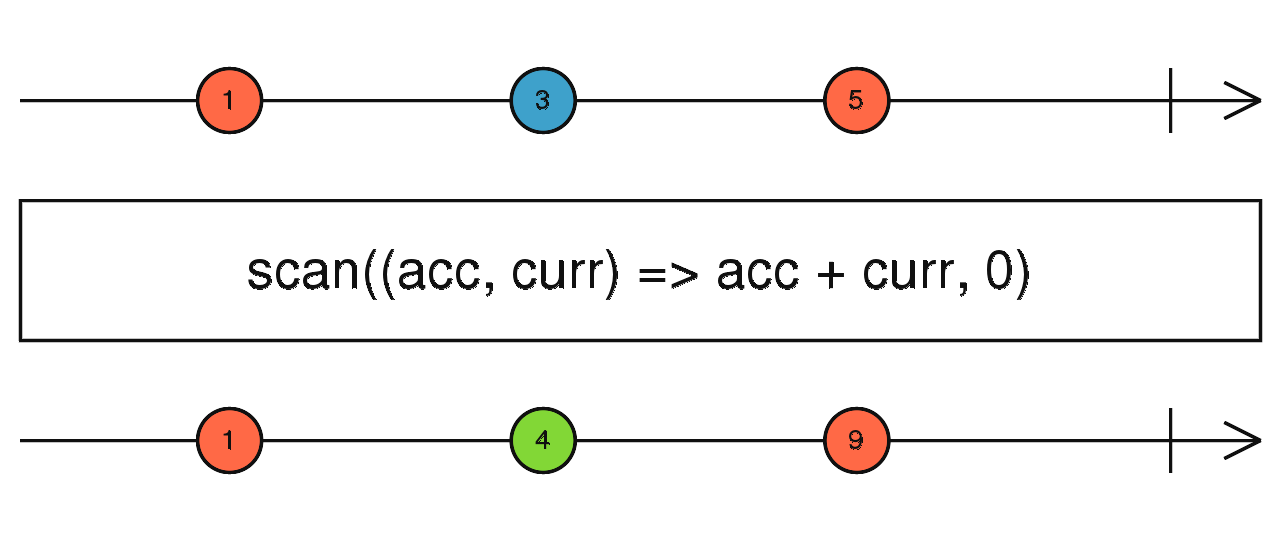
\includegraphics[width=\linewidth]{scan}
            \end{frame}

            \subsubsection{.tap()}\label{subsub:tap}

            \begin{frame}{\insertsubsectionhead}{\nameref{subsub:observable}}
                \begin{block}{\texttt{\insertsubsubsectionhead} (precedentemente \texttt{.do()})}
                    \begin{itemize}
                        \item
                            la versione ``\engEmph{pipable}'' è stata rinominata da \texttt{.do()} a \texttt{.tap()} per conflitto di nomi con funzioni standard di JavaScript
                        \item
                            esegue un \engEmph{side effect} per ogni valore emesso dall'\texttt{Observable} sorgente, ma lo ritorna invariato
                        \item
                            estremamente utile in fase di debug
                    \end{itemize}
                \end{block}
            \end{frame}

            \begin{frame}[fragile]{\insertsubsectionhead}{\nameref{subsub:observable}: Pipable operators: \texttt{\insertsubsubsectionhead}}
                \inputminted{js}{src/tap.js}
                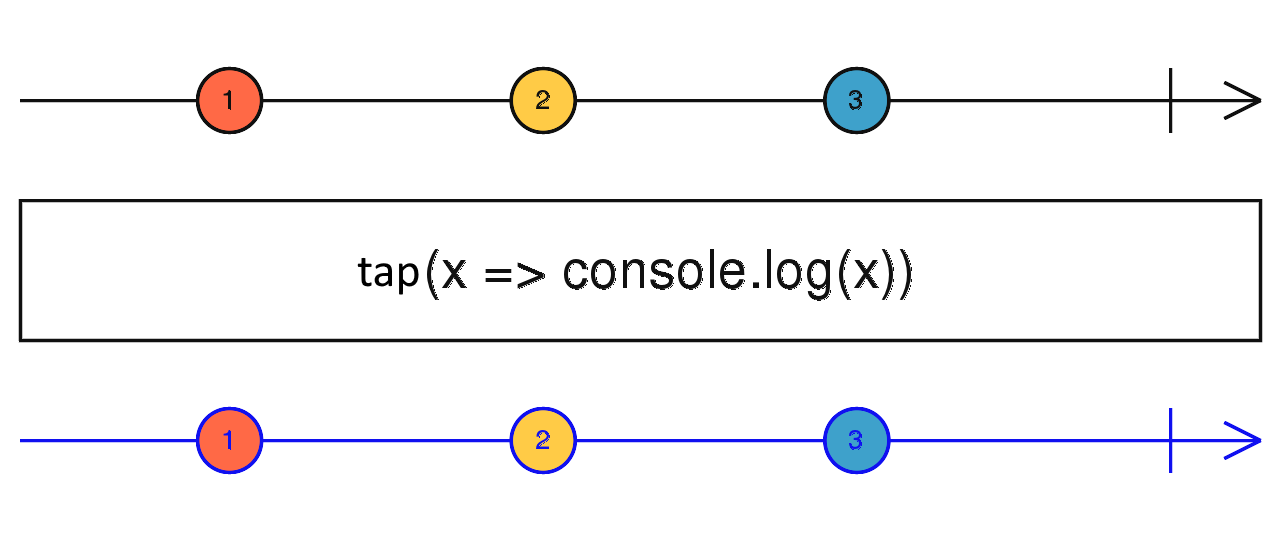
\includegraphics[width=\linewidth]{tap}
            \end{frame}

            \subsubsection{.debounce() \& .debounceTime()}\label{subsub:debounce}

            \begin{frame}{\insertsubsectionhead}{\nameref{subsub:observable}}
                \begin{block}{\texttt{\insertsubsubsectionhead}}
                    \begin{itemize}
                        \item
                            Permettono di filtrare gli eventi emessi dall'\texttt{Observable} sorgente, emettendo un valore solo dopo che è passato un certo numero di millisecondi da quando non sono stati emessi valori
                        \item
                            \texttt{.debounceTime()} permette di specificare il lasso di tempo entro il quale effettuare il \engEmph{debounce}
                        \item
                            \texttt{.debounce()} si comporta come \texttt{.debounceTime()}, ma il periodo di silenzio è determinato da un altro \texttt{Observable}
                        \item
                            utili per attendere che l'utente abbia terminato di fare qualcosa con un componente osservato prima di gestire l'evento
                    \end{itemize}
                \end{block}
            \end{frame}

            \begin{frame}[fragile]{\insertsubsectionhead}{\nameref{subsub:observable}: Pipable operators: \texttt{.debounceTime()}}
                % \inputminted{js}{src/debounceTime.js}
                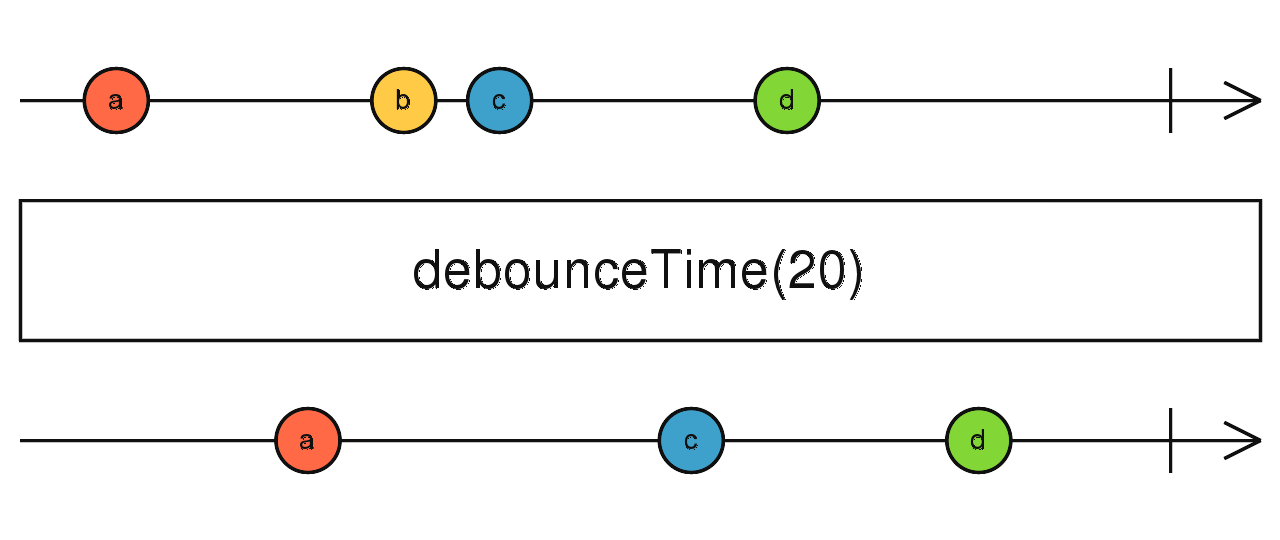
\includegraphics[width=\linewidth]{debounceTime}
            \end{frame}

            \subsubsection{.throttle() \& .throttleTime()}\label{subsub:throttle}

            \begin{frame}{\insertsubsectionhead}{\nameref{subsub:observable}}
                \begin{block}{\texttt{\insertsubsubsectionhead}}
                    \begin{itemize}
                        \item
                            Permettono di filtrare gli eventi emessi dall'\texttt{Observable} sorgente, emettendo un valore solo ogni un certo lasso di tempo
                        \item
                            \texttt{.throttleTime()} emette un valore dall'\texttt{Observable} sorgente ed ignora ulteriori valori per i millisecondi specificati
                        \item
                            \texttt{.throttle()} si comporta come \texttt{.throttleTime()}, ma il periodo di silenzio è determinato da un altro \texttt{Observable}
                        \item
                            utili per ridurre il numero di input a livelli accettabili
                    \end{itemize}
                \end{block}
            \end{frame}

            \begin{frame}[fragile]{\insertsubsectionhead}{\nameref{subsub:observable}: Pipable operators: \texttt{.throttleTime()}}
                % \inputminted{js}{src/throttleTime.js}
                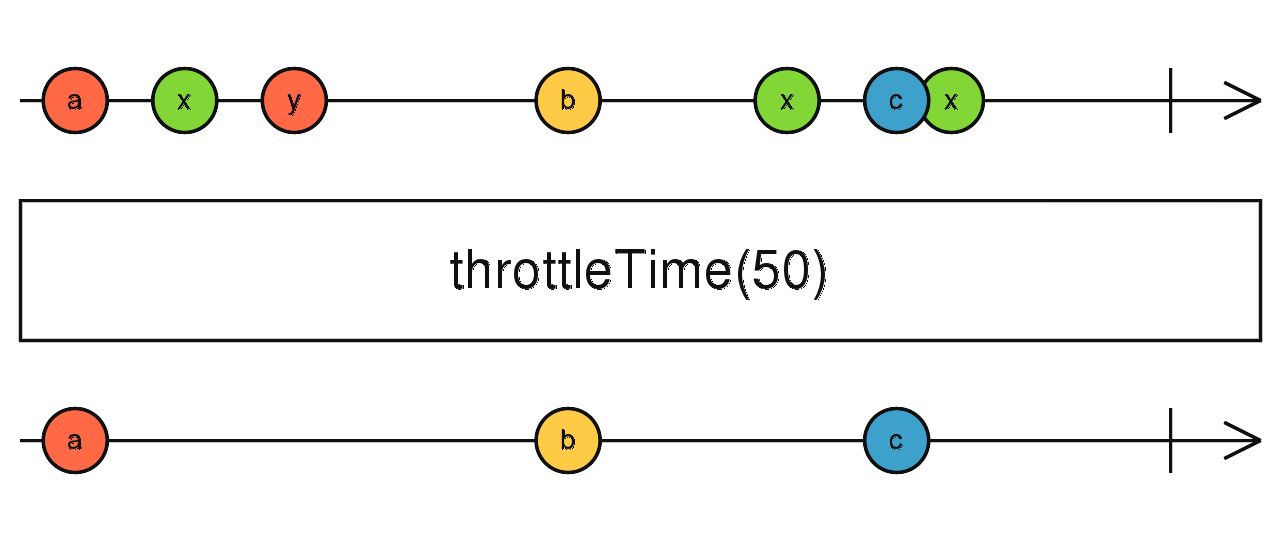
\includegraphics[width=\linewidth]{throttleTime}
            \end{frame}

            \subsubsection{.catchError()}\label{subsub:catch}

            \begin{frame}{\insertsubsectionhead}{\nameref{subsub:observable}}
                \begin{block}{\texttt{\insertsubsubsectionhead} (precedentemente \texttt{.catch()})}
                    \begin{itemize}
                        \item Pippo
                    \end{itemize}
                \end{block}
            \end{frame}

            \subsubsection{Subject}\label{subsub:subject}

            \begin{frame}{\insertsubsectionhead}
                \begin{block}{\texttt{\insertsubsubsectionhead}}
                    \begin{itemize}
                        \item Topolino
                    \end{itemize}
                \end{block}
            \end{frame}

    \nocite{*}
    \section{\refname}\label{sec:ref}
    \begin{frame}[t,allowframebreaks]
        \frametitle{\insertsectionhead}
        \printbibliography
    \end{frame}
\end{document}
